\documentclass[journal]{IEEEtran}

\usepackage{amsmath}
\usepackage{amssymb}
\usepackage{booktabs}
\usepackage{graphicx}
\usepackage{cite}
\usepackage{url}
\usepackage{algorithm}
\usepackage{algorithmic}
\usepackage{array}

\title{Three-Tree Genetic Programming for Skill-Based Peer Coordination in Multi-Site Inventory Control}
\author{Author~Name}

\begin{document}
\maketitle

\begin{abstract}
Multi-site inventory control requires local replenishment decisions and
coordinated lateral transfers under uncertain demand. Treating every transfer
pair independently can allocate the same donor stock more than once, while
giving a central policy unrestricted access to all site states obscures the
information requirements of coordination. This paper develops a reproducible
method in which each site is a peer inventory agent with local observations,
explicit decision skills, and a reservation ledger. An offline genetic
programming (GP) search evolves a shared individual with exactly three
expression trees: replenishment, support request, and support offer. Fixed skill
wrappers interpret these expressions as bounded quantities. A non-evolved
protocol exchanges forecast-slack summaries, evaluates candidate quantities,
confirms mutually preferred partners over a finite number of rounds, and
reserves quantities without a central matching optimizer. Negotiation precedes
current demand realization; its output is therefore a conditional commitment,
not an executed transfer. After demand and due arrivals, a physical executor
revalidates donor stock and receiver capacity and records actual dispatches
separately from promises. This manuscript specifies the GP representation,
agent--skill relationship, fixed negotiation, and simulator-grounded evaluation.
The fixed gain is a forecast-based heuristic, not a calibrated value function
or a guarantee of optimality. Comparative performance and industrial
generalization remain empirical questions.
\end{abstract}

\begin{IEEEkeywords}
Genetic programming, multi-agent coordination, inventory control, lateral
transshipment, interpretable decision rules.
\end{IEEEkeywords}

\section{Introduction}
Multi-location inventory systems couple decisions that appear local:
an order changes future availability, and a transfer improves one site's
position while consuming another site's stock. Classical inventory policies
provide important interpretable baselines \cite{zipkin2000foundations,axsater2015inventory},
while lateral transshipment introduces interactions among inventory positions,
costs, and service requirements \cite{paterson2011lateral}.
The present setting concerns sites belonging to one enterprise. They share a
system-cost objective but retain local information, inventory responsibilities,
and service targets. No monetary bargaining between independent firms is
assumed.

GP searches executable symbolic policies rather than prescribing their final
algebraic structure \cite{koza1992genetic,poligp2008fieldguide}.
However, directly returning one signed quantity for every site pair does not
by itself define a decentralized coordination process. Simultaneous pairwise
decisions may compete for the same stock; an accepted proposal may also become
infeasible when demand is realized before dispatch.
These issues motivate an explicit separation of policy representation,
agent authority, and protocol execution.

We study three-tree GP with fixed peer negotiation. Each site executes the
same evolved policy on its own observation. Replenishment, request, and offer
skills use distinct GP trees, whereas routing, partner confirmation,
reservations, and feasibility checks are fixed mechanisms. Offline team
evaluation can be centralized without making online decisions centralized:
agents exchange only specified summaries, and no agent commands another
site's transfer.

The method is intended to support three investigations:
\begin{enumerate}
    \item whether a request--offer representation with explicit commitments
    improves coordination relative to independent pairwise transfer rules;
    \item whether GP can discover useful local replenishment, request, and
    offer expressions under the same fixed negotiation protocol;
    \item how finite communication rounds, topology, and conditional execution
    affect cost and site-level service.
\end{enumerate}
These are testable questions, not claims of established superiority.
The implementation and editable diagrams accompany this methods draft.

\section{Background and Scope}
Inventory rules, simulation optimization, and symbolic policy search are
complementary. Classical policies expose understandable stock targets;
simulation can represent stochastic transitions and operational constraints
\cite{amaran2016simulation}; GP can search nonlinear expressions without a
differentiable simulator. A GP tree is a decision expression, not an autonomous
agent. Autonomy additionally requires an observation boundary, memory,
permitted messages, and authority over local actions.

Likewise, peer agreement is not synonymous with numerical consensus in
networked control \cite{olfati2007consensus}. Here agreement means that two
endpoints confirm the same conditional transfer within a finite-round
protocol. We make no asymptotic convergence, strategy-proofness, privacy, or
globally optimal matching claim. A skill is a callable decision module with
preconditions, output bounds, and execution feedback; it is not necessarily a
temporally extended reinforcement-learning option.

\section{Problem and Information Structure}
\label{sec:problem}
Consider $N\geq 2$ inventory sites on a configured undirected graph
$\mathcal G=(\mathcal V,\mathcal E)$. At the start of period $t$, site $i$
observes its on-hand inventory $I_i$, outstanding order pipeline $P_i$,
forecast vector $\hat{\mathbf d}_i$, storage capacity $Cap_i$, and operating
cost parameters. It also maintains current-period commitments and an
execution history. Let $h_i$, $b_i$, $a_i$, and $k_i$ denote holding,
lost-sales, unit-order, and fixed-order costs. A dispatched transfer incurs
unit cost $c^{tr}$ and fixed cost $K^{tr}$.

An agent cannot inspect another site's simulator object, current realized
demand, future realized demand, or a full-network inventory aggregate.
Neighbor communication exposes only the specified request/offer summaries,
cost coefficients, and commitment updates. Such summaries are not a formal
privacy mechanism.

\subsection{Decision and Execution Timing}
The timing is intentionally retained from the replenish-and-transship
benchmark: agents choose orders and negotiate before observing current
realized demand. The environment subsequently applies due arrivals and
demand, revalidates transfers, charges costs, and advances the pipeline.
Consequently, a promised quantity is not automatically deliverable.

Let $A_i(t)$ be due arrivals and $D_i(t)$ realized demand. Before physical
transfers,
\begin{equation}
    z_i(t)=\min\{Cap_i,I_i(t)+A_i(t)\}-D_i(t).
\end{equation}
For a directed commitment $i\rightarrow j$ with planned quantity $q^p$,
the executor can dispatch no more than
\begin{equation}
    q^e=\min\{q^p,\max(0,z_i),\max(0,Cap_j-z_j)\},
    \label{eq:execution}
\end{equation}
with $z_i,z_j$ updated after preceding dispatches. The implementation uses a
documented deterministic dispatch order. This introduces an execution-order
effect when resources change after commitment; it is not claimed to remove
all allocation bias. Zero, partial, and full dispatches are distinguished.

After transfers, negative inventory is charged as unmet demand and reset to
zero. Positive inventory incurs holding cost. Order decisions enter the
pipeline according to the benchmark lead-time convention. Receiver capacity
is enforced at physical dispatch, not merely at proposal generation.
The complete observable pipeline has $L_o$ slots: its head arrives in the
current period, then the pipeline shifts and the new order is appended.
Thus an order chosen in period $t$ arrives in period $t+L_o$; with
$L_o=2$, the first order arrives in period 3. This is physically equivalent
to the inherited simulator's shorter queue plus separately staged action.
The new policy interface explicitly exposes all outstanding orders, so
baseline comparisons must align pipeline information as well as dynamics.
Overflow at a capped arrival is discarded and measured.

\subsection{Objective and Measurements}
The period cost is
\begin{align}
 C_t={}&\sum_{i\rightarrow j}
 \left(c^{tr}q^e_{ij}+K^{tr}\mathbb I[q^e_{ij}>0]\right) \nonumber\\
 &+\sum_i\left(h_i\max(z_i,0)+b_i\max(-z_i,0)\right) \nonumber\\
 &+\sum_i\left(a_i x_i+k_i\mathbb I[x_i>0]\right).
\end{align}
The episode objective is realized cost divided by the actual number of
simulated periods. Service is measured using unmet demand units and demand
fill rate, not a count of zero ending inventories.

Synthetic demand uses stochastic Poisson realizations conditional on the
benchmark's exposed demand means. These mean forecasts are privileged model
information and should not be interpreted as evidence of real forecasting
accuracy. Historical records copied into future forecast slots constitute
an oracle setting; they must be explicitly marked or rejected, rather than
silently presented as causal forecasting.
Synthetic episodes retain the inherited reset convention: the stream seed
is the supplied episode seed plus 1000. Shortened execution horizons do not
regenerate a different demand table.

\section{Three-Tree GP with Fixed Peer Negotiation}
\label{sec:method}

\subsection{GP, Agent, and Skill Are Different Objects}
An \emph{agent} is the persistent site-level decision entity: it owns local
observations, inventory responsibilities, neighbor interfaces, reservations,
and execution memory. A \emph{skill} is a bounded callable module within that
agent. A \emph{GP tree} is the symbolic expression used by a particular
decision skill. GP itself is the offline search procedure that changes the
expressions. None of these objects requires an LLM.

The population individual is the ordered tuple
\begin{equation}
    \Theta=(T^{ord},T^{req},T^{off}),
    \label{eq:individual}
\end{equation}
containing exactly three trees. The same $\Theta$ is deployed at every site,
but each invocation receives a different local observation. This is shared
parameterization, not shared access to site states.

\begin{figure*}[t]
    \centering
    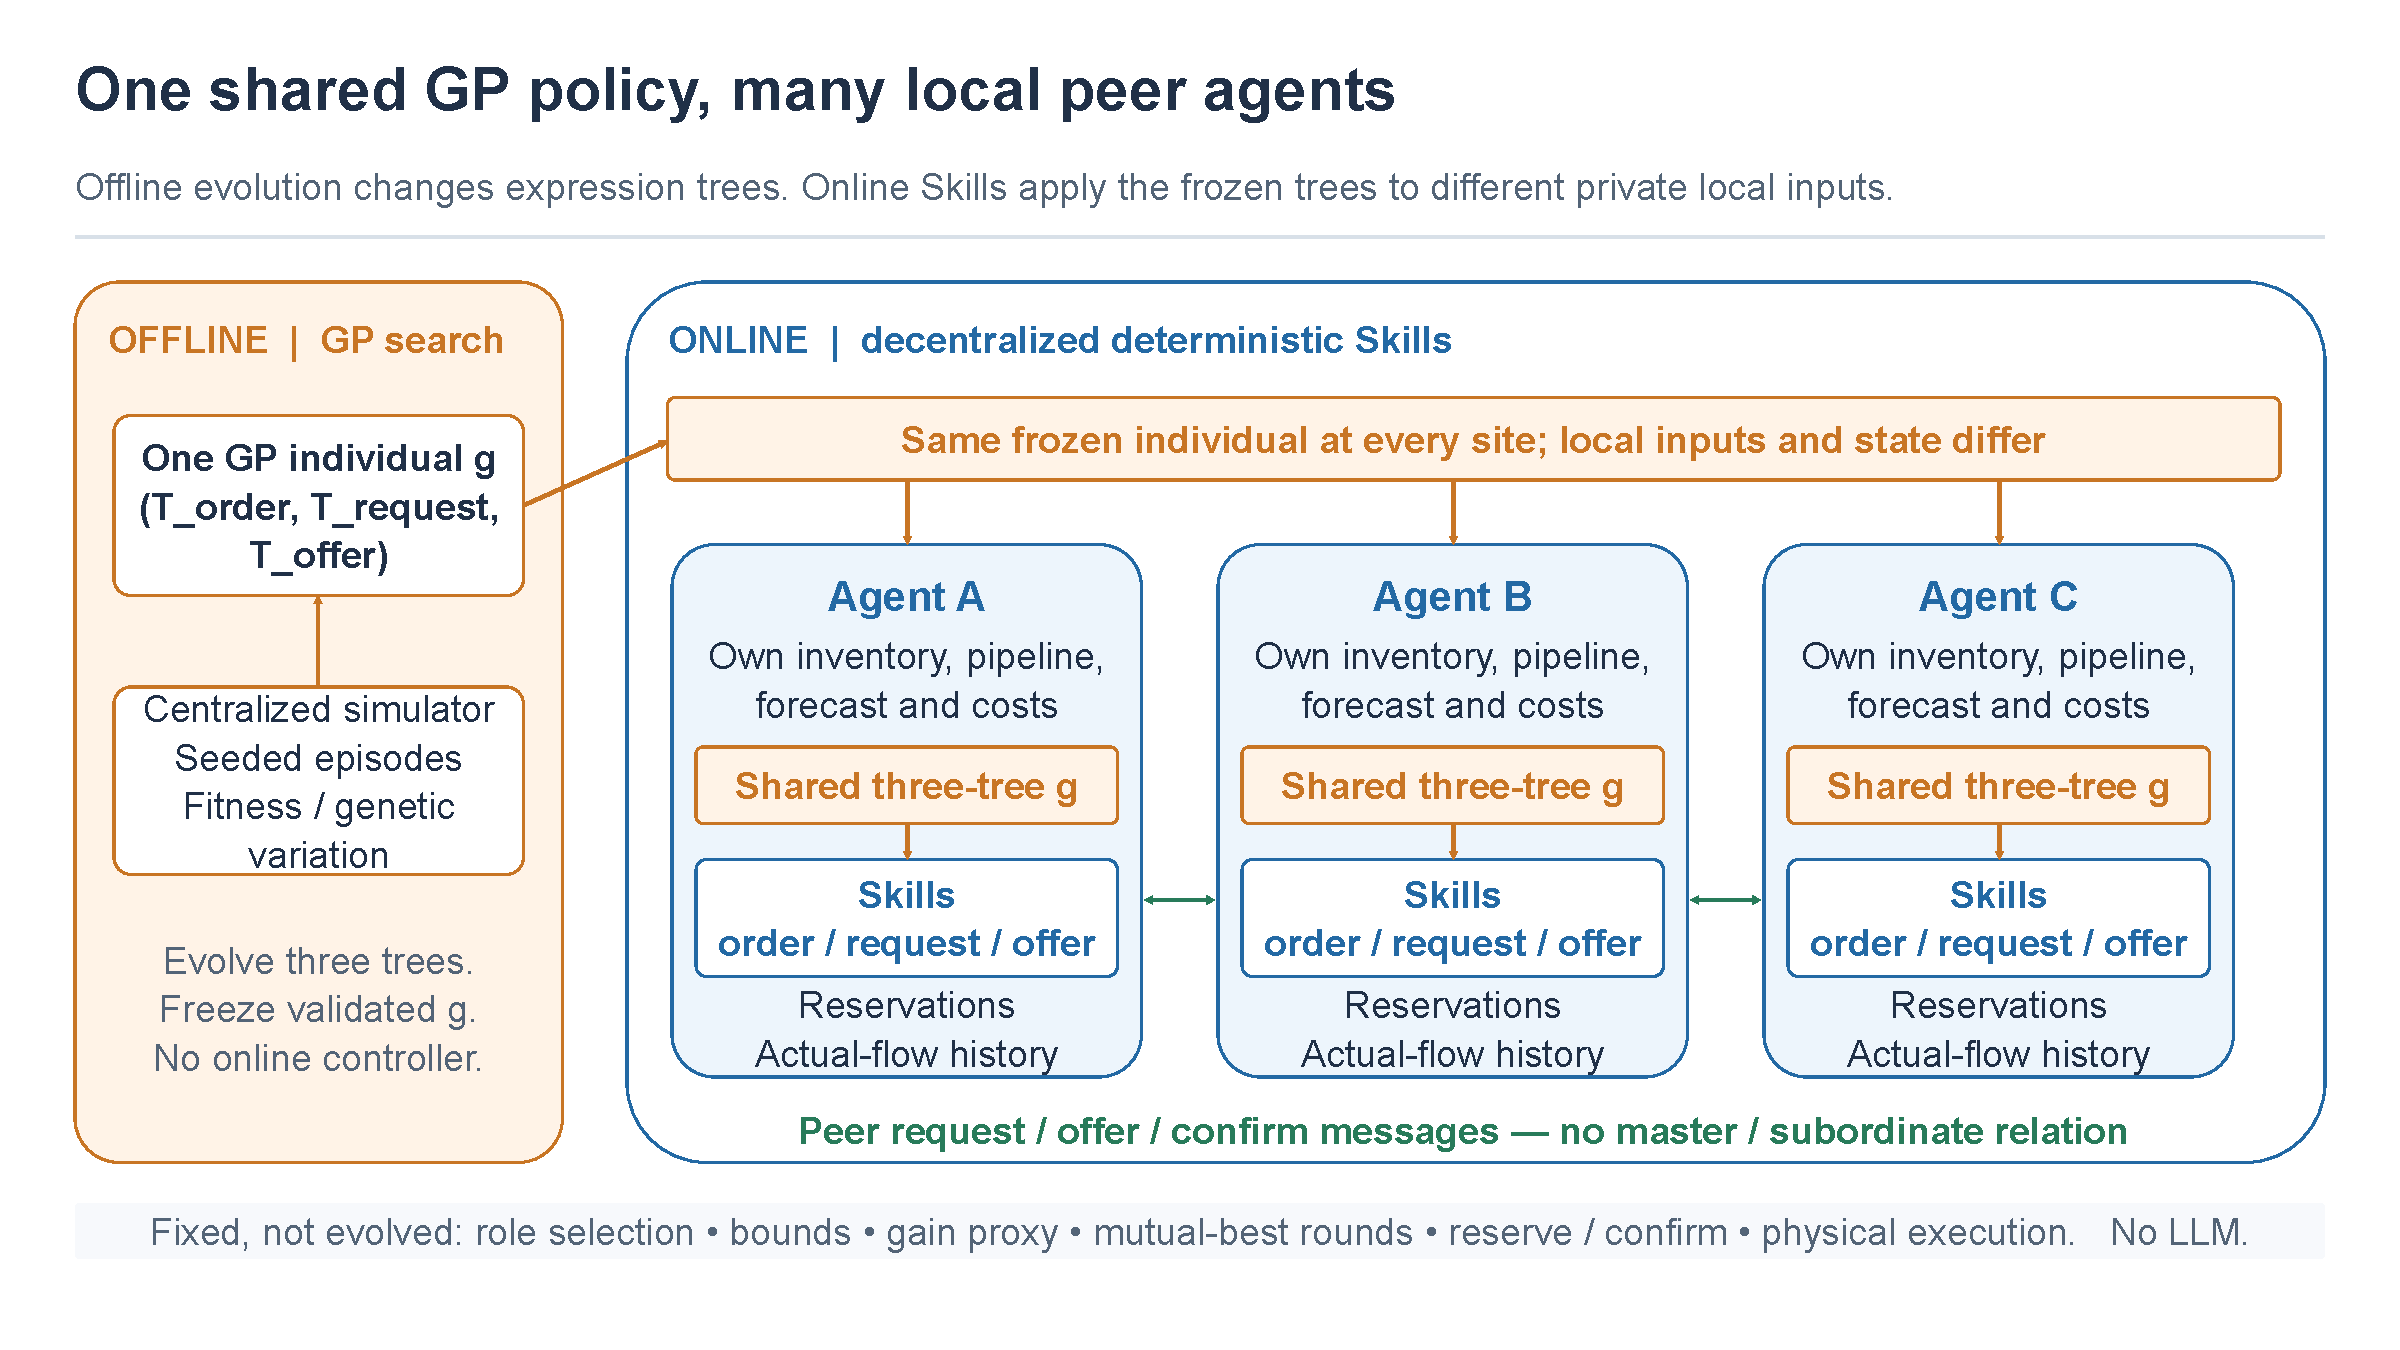
\includegraphics[width=0.96\textwidth]{figures/gp_agent_skills/architecture.pdf}
    \caption{Relationship between offline GP, the shared three-tree individual,
    site agents, and their decision skills. Fixed protocol and physical
    execution mechanisms are outside the evolved representation.}
    \label{fig:architecture}
\end{figure*}

Table~\ref{tab:boundaries} separates evolved and fixed responsibilities.
\begin{table}[t]
\centering
\caption{Responsibility boundaries}
\label{tab:boundaries}
\footnotesize
\begin{tabular}{p{0.24\linewidth}p{0.66\linewidth}}
\toprule
Object & Responsibility \\
\midrule
$T^{ord}$ & Compute a raw local replenishment quantity. \\
$T^{req}$ & Compute a raw support-request quantity. \\
$T^{off}$ & Compute a raw support-offer quantity. \\
Skill wrapper & Supply allowed features, validate numeric outputs, apply
nonnegativity and operational bounds. \\
Agent & Maintain local observation, routing identity, role, commitments,
and actual execution memory. \\
Fixed protocol & Exchange summaries, score quantity candidates, select
mutual partners, reserve and confirm. \\
Physical executor & Apply arrivals and demand; recheck stock/capacity;
record actual transfers and costs. \\
\bottomrule
\end{tabular}
\end{table}

\subsection{Local Features and Skill Outputs}
The GP feature interface contains local inventory and pipeline summaries,
exposed forecasts, capacity and cost parameters, and explicitly available
previous-period execution features. Features are named, so a tree's
terminal meaning is independent of a legacy array position. Raw neighbor
states, hidden demand samples, and global inventory totals are excluded.
Site identities are used for routing and deterministic tie-breaking, not as
GP decision terminals.

\begin{table}[t]
\centering
\caption{Exact named GP terminal sets}
\label{tab:terminals}
\footnotesize
\begin{tabular}{p{0.18\linewidth}p{0.72\linewidth}}
\toprule
Scope & Terminals \\
\midrule
All trees & \texttt{I, PIPE, DUE, F, FC1, FC2, CAP, H, B, RHO,
LAST\_IN, LAST\_OUT, LAST\_LOST} \\
Order only & \texttt{ORDER\_FIXED, ORDER\_UNIT} \\
Request only & \texttt{ROOM, DEFICIT, TC, TK} \\
Offer only & \texttt{AVAIL, SURPLUS, TC, TK} \\
\bottomrule
\end{tabular}
\end{table}
\texttt{PIPE} includes all previously placed outstanding orders;
\texttt{DUE} is the first pipeline entry. \texttt{F} sums all exposed means,
whereas \texttt{FC1} and \texttt{FC2} are the first two entries
(\texttt{FC2} is zero if absent). The three \texttt{LAST} terminals refer to
actual received, sent, and lost quantities in the preceding period; they
start at zero. Transfer costs \texttt{TC,TK} are public scenario parameters.
No site-ID, time-index, topology, or production-capacity terminal is used.

Let $f_i$ denote the allowed feature vector. Fixed wrappers convert tree
outputs to bounded quantities:
\begin{align}
    x_i &= \operatorname{clip}(T^{ord}(f_i),0,U_i^{ord}),\\
    r_i &= \operatorname{clip}(T^{req}(f_i),0,U_i^{req}),\\
    s_i &= \operatorname{clip}(T^{off}(f_i),0,U_i^{off}).
    \label{eq:skill-outputs}
\end{align}
The bounds are derived from the configured benchmark and current role;
they are not additional learned trees. Orders are capped by storage
capacity per order, not by currently empty storage space. A supply bound at
negotiation time is not a guarantee of available stock after demand.

Define forecast exposure and forecast slack by
\begin{equation}
 F_i=\sum_{\kappa}\hat d_i^{(\kappa)},\qquad
 \rho_i=I_i+\sum P_i-F_i.
 \label{eq:slack}
\end{equation}
With $\epsilon=10^{-8}$, role assignment is fixed: a site with
$\rho_i>\epsilon$ can offer, one with $\rho_i<-\epsilon$ can request,
and other sites are inactive. Exact bounds are
\begin{align}
 U_i^{ord}&=Cap_i,\\
 U_i^{req}&=\min\{\max(0,-\rho_i),\max(0,Cap_i-I_i)\},\\
 U_i^{off}&=\min\{\max(0,\rho_i),\min(Cap_i,I_i+P_i[0])\}.
\end{align}
Inactive-role request/offer quantities are zero. Due arrivals enter the
conditional supply bound; other pipeline entries only affect forecast
slack. The implementation excludes receiving and forwarding within the
same period. A GP output of zero can decline participation even when the
role permits it.

The observation, GP features, period role, and initial skill quantities
remain frozen during negotiation. Trees are not reevaluated after each
match; only message quantities and reservation-adjusted slack change.
An order newly selected in the current period does not enter that period's
observed pipeline or slack.

\subsection{Expression Representation and Example}
Each tree is a prefix expression with six binary primitives:
\texttt{add, sub, mul, div, maximum, minimum}. Search constants are
$\{0,0.25,0.5,1,2\}$. GP terminal inputs and primitive results are saturated
to $[-10^6,10^6]$. Protected division returns $1$ when the denominator's
absolute value is at most $10^{-8}$; otherwise the quotient is saturated.
Physical state, skill bounds, messages, and proxy gains are not subjected
to this GP numeric saturation. Nonfinite policy values raise an explicit
numerical-policy error. These are numeric expression trees, not a
dimensionally typed program language.

An illustrative valid individual is
\begin{align}
 T^{ord}(f_i)&=\max(0,F_i-I_i-\sum P_i),\\
 T^{req}(f_i)&=\max(0,F_i-I_i-\sum P_i),\\
 T^{off}(f_i)&=\max(0,I_i-F_i).
\end{align}
This is an expression example, not the exact initialized seed and not a
reported evolved optimum. Its order and request
expressions are identical but have different execution roles: the former
orders material with a lead time, whereas the latter advertises demand for
peer support. Fixed caps still apply. Figure~\ref{fig:individual} shows the
three-tree structure.

\begin{figure*}[t]
    \centering
    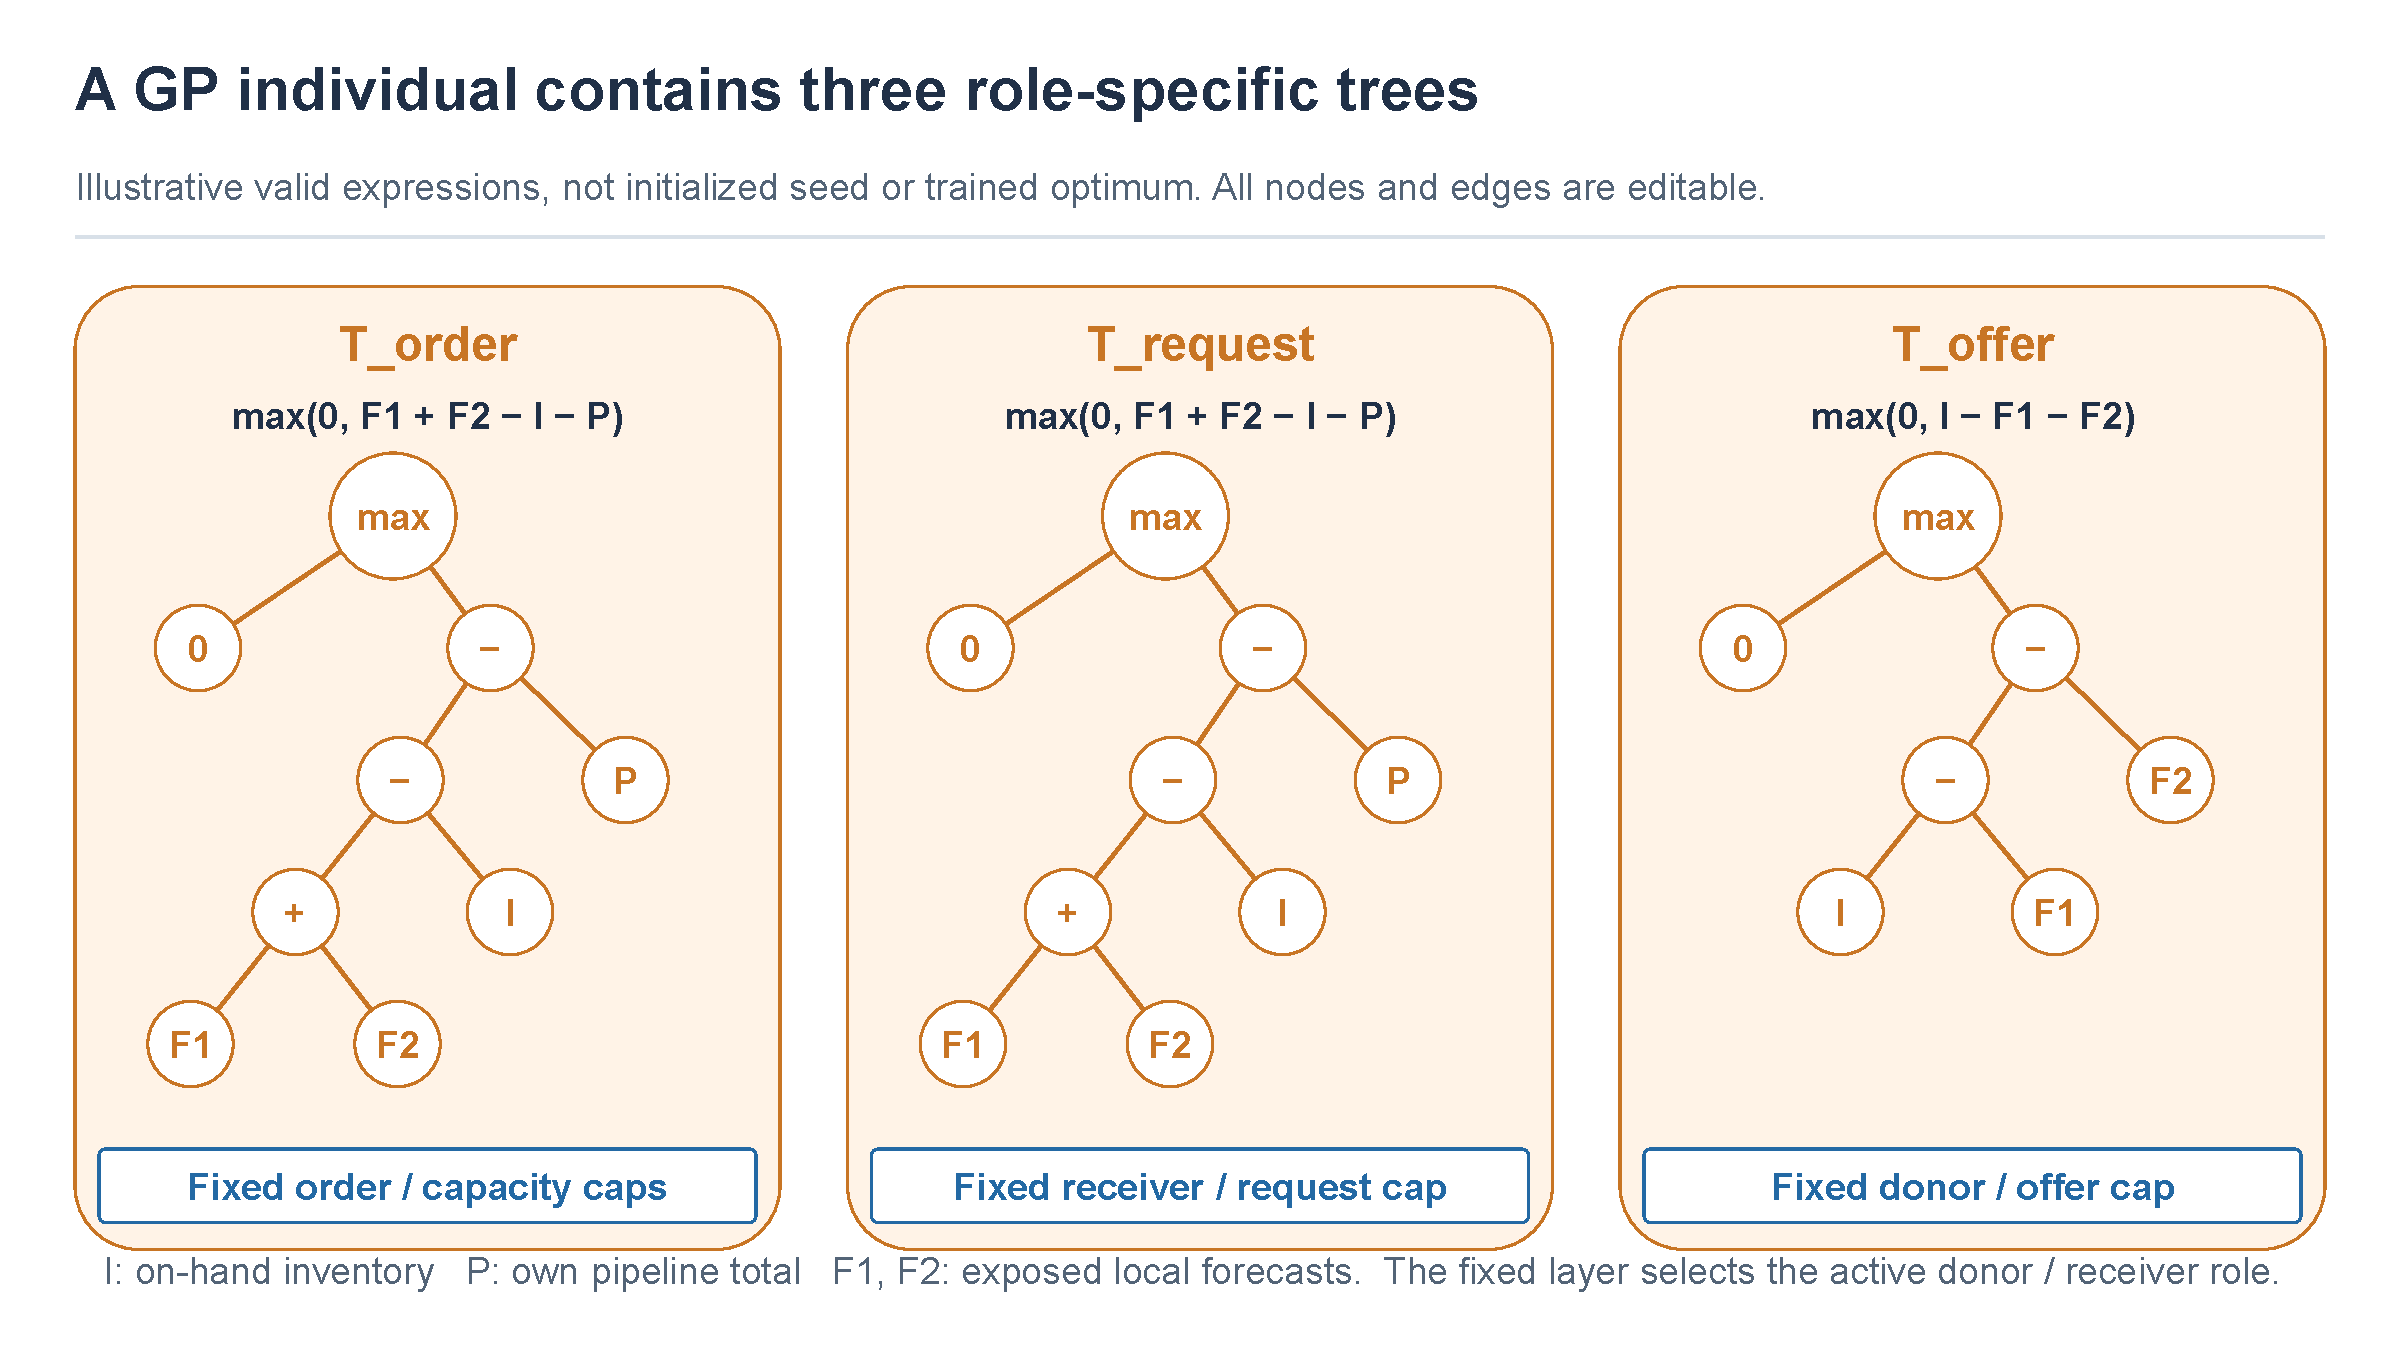
\includegraphics[width=0.96\textwidth]{figures/gp_agent_skills/gp_individual.pdf}
    \caption{An illustrative three-tree individual. Trees encode expressions;
    skills supply semantics, bounds, and lifecycle. The diagrams remain
    editable in the accompanying PowerPoint deck.}
    \label{fig:individual}
\end{figure*}

\subsection{Messages and Fixed Quantity Evaluation}
An agent sends request or offer quantities and the forecast-slack/cost
summary required by the protocol to its configured neighbors. Current-period
commitments reduce the remaining advertised request/supply and adjust
effective slack for subsequent negotiation rounds. Neither endpoint needs
to query the other's simulator object.

The non-evolved local proxy is
\begin{equation}
    \Phi_i(\rho)=h_i\max(\rho,0)+b_i\max(-\rho,0).
\end{equation}
For a candidate quantity $q$ from donor $i$ to receiver $j$,
\begin{align}
 A_i(q)&=\Phi_i(\rho_i-q)-\Phi_i(\rho_i),\\
 B_j(q)&=\Phi_j(\rho_j)-\Phi_j(\rho_j+q),\\
 G_{ij}(q)&=B_j(q)-A_i(q)-c^{tr}q
              -K^{tr}\mathbb I[q>0].
 \label{eq:gain}
\end{align}
The gain is a deterministic forecast-slack heuristic. It is not an unbiased
estimate of future cost, a donor-shortage probability, or an incentive
compatibility condition. Its fixed definition deliberately isolates the
contribution of evolving the three quantity trees.

Let $\bar s_i$ and $\bar r_j$ be remaining quantities after reservations.
The protocol evaluates a small grid:
\begin{equation}
 \mathcal Q_{ij}=
 \left\{\eta\min(\bar s_i,\bar r_j):
       \eta\in\{0,\tfrac14,\tfrac12,\tfrac34,1\}\right\}.
\end{equation}
For each ascending grid fraction, the implementation computes
$q=\min\{q_{\max},\operatorname{round}(\eta q_{\max},6)\}$, where
$q_{\max}=\min(\bar s_i,\bar r_j)$. Rounding uses ties-to-even; clipping
after rounding cannot exceed the remaining budget. Candidates are deduplicated
within $10^{-8}$. Orders, initial skill budgets, and actual dispatch quantities
are otherwise not rounded.
Only $q>10^{-8}$ and $G_{ij}(q)>10^{-8}$ are eligible.
Common ranking is gain descending, donor ID ascending, receiver ID ascending,
then quantity descending; gains are compared exactly.

The conservative surplus/deficit caps have an important consequence:
no candidate crosses the proxy's donor or receiver breakpoint. Thus,
\begin{align}
 A_i(q)&=-h_iq,\qquad B_j(q)=b_jq,\\
 G_{ij}(q)&=(h_i+b_j-c^{tr})q-K^{tr}.
\end{align}
Whenever an eligible candidate exists, the largest available grid quantity
is preferred. The grid is therefore not discovering an interior nonlinear
risk optimum in this version. GP still controls advertised budgets, which
change edge limits, gains, partner choices, and commitments.

\begin{figure*}[t]
    \centering
    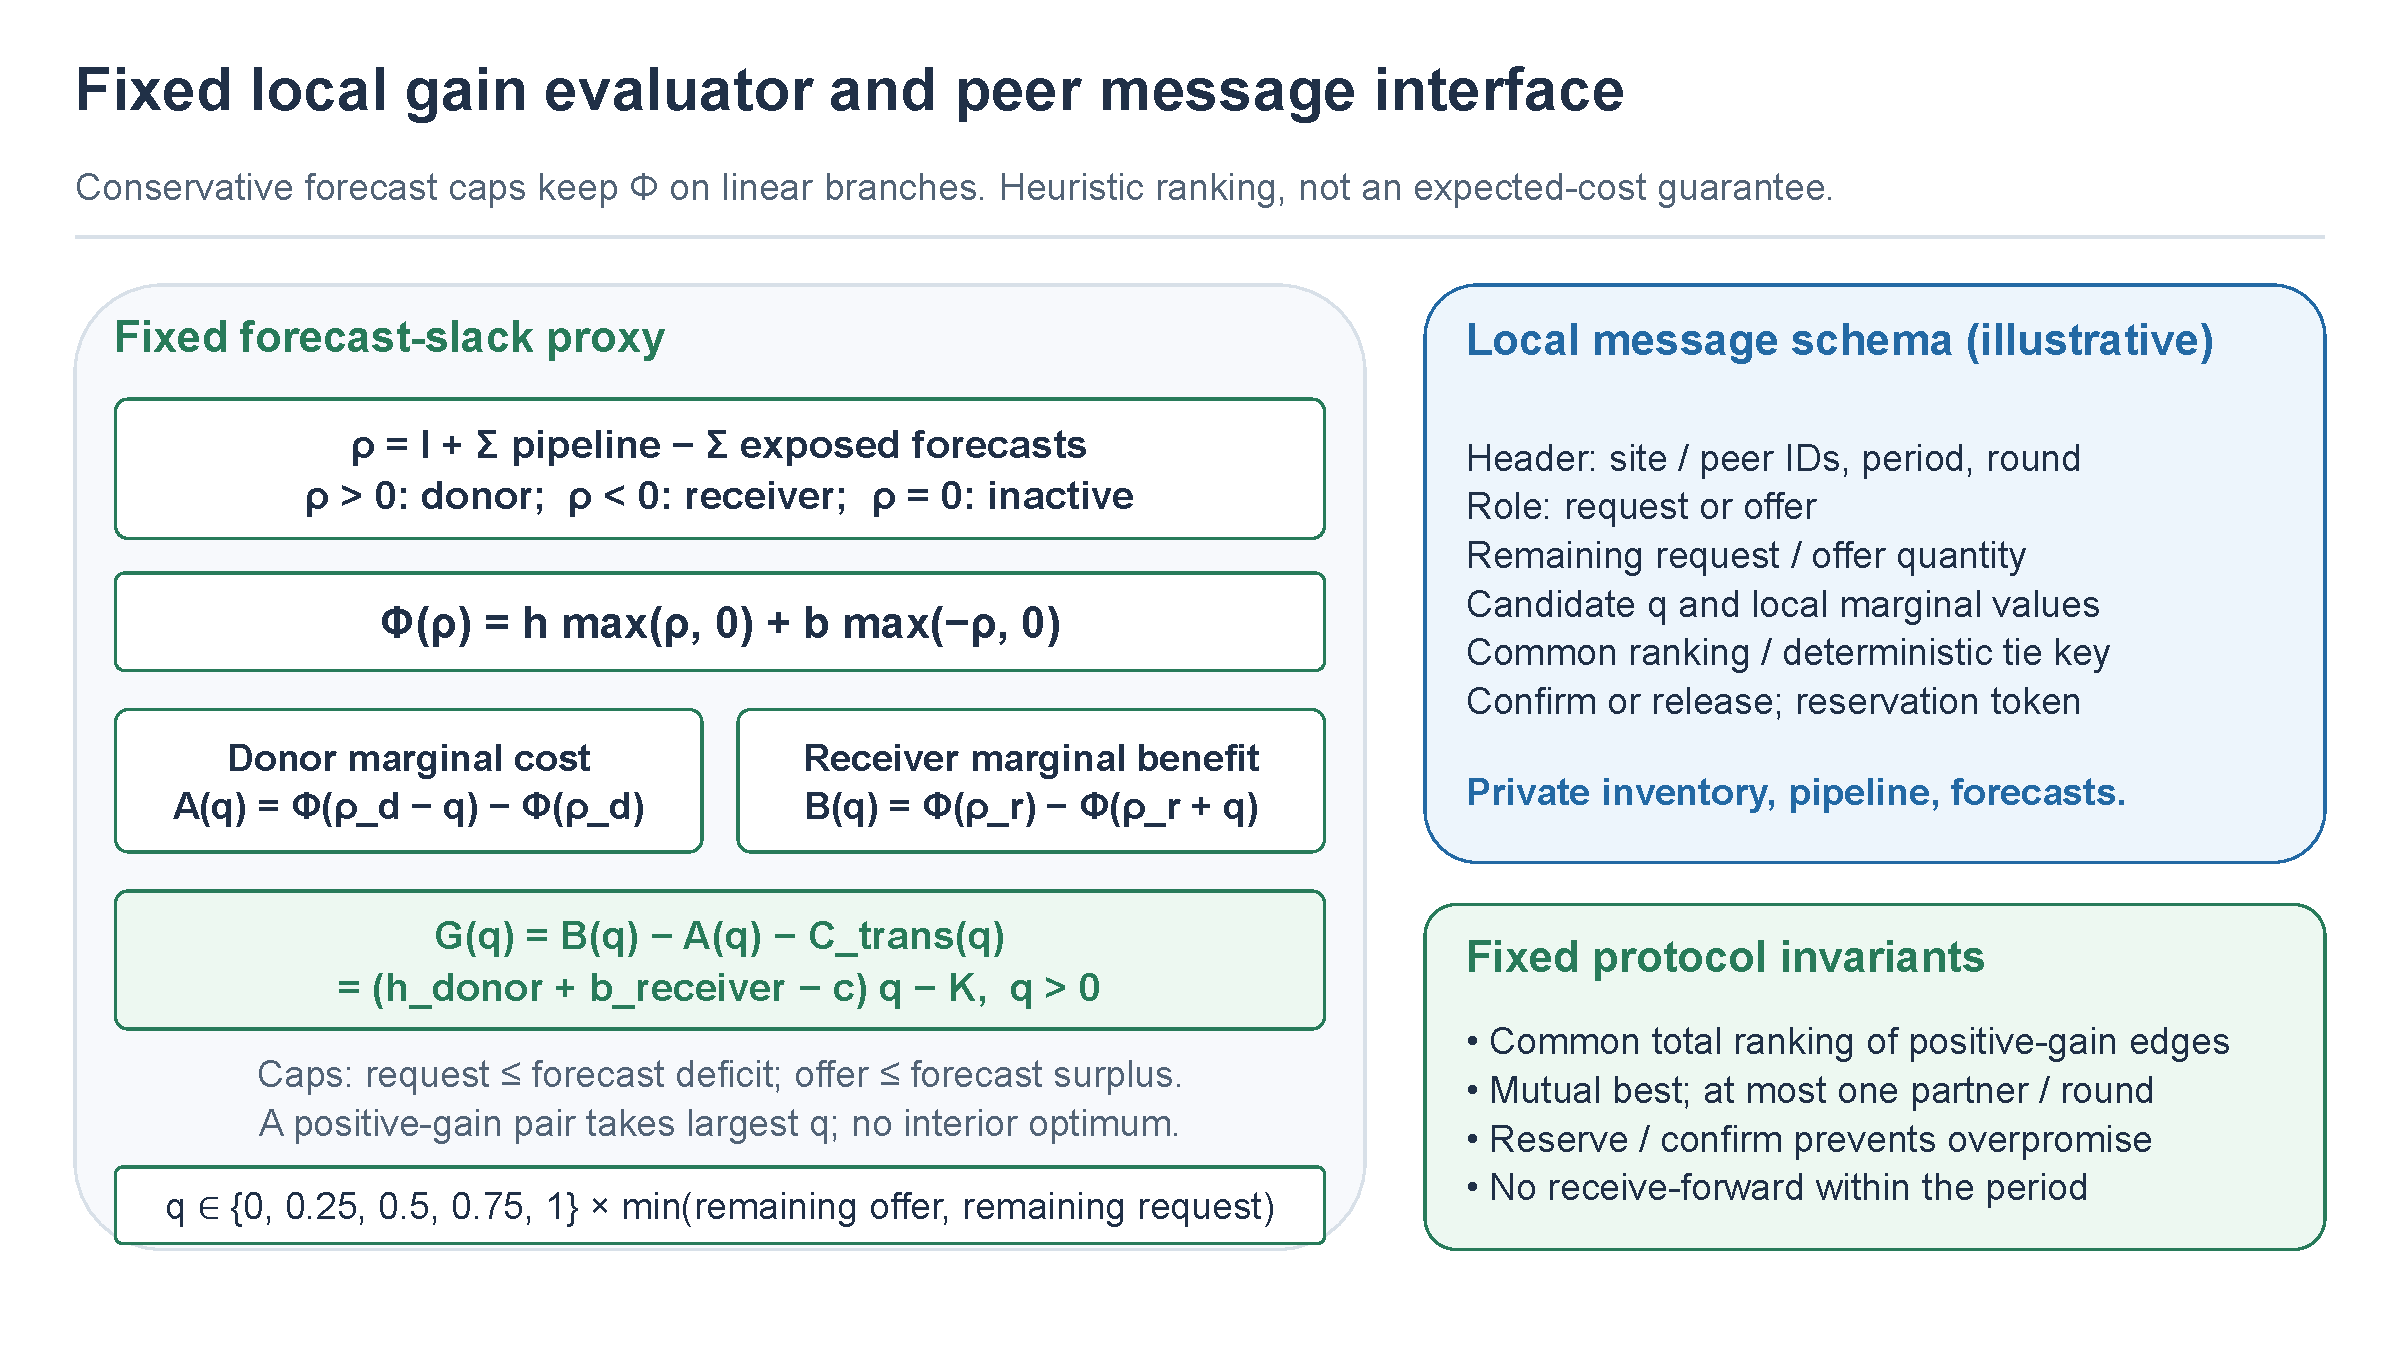
\includegraphics[width=0.96\textwidth]{figures/gp_agent_skills/fixed_evaluator.pdf}
    \caption{The fixed evaluator uses advertised summaries to score a finite
    quantity grid. It is not an evolved fourth tree or an online LLM.}
    \label{fig:evaluator}
\end{figure*}

\subsection{Finite-Round Mutual Matching and Reservations}
Independent bilateral acceptance can over-commit a donor. Instead, in each
round every active agent chooses its highest-ranked eligible incident edge.
An edge is confirmed only when its endpoints choose one another. A common
ranking combines predicted gain and deterministic identifiers, so endpoints
agree on tie resolution.

Each site can confirm at most one partner in a round, but may confirm
different partners over successive rounds while resources remain.
Confirmation immediately updates both ledgers and the advertised remaining
quantities. The protocol terminates after the configured round limit or
when no additional mutual match exists. A simulator can deliver messages
synchronously without acting as a global matching optimizer.

\begin{algorithm}[t]
\caption{Fixed peer negotiation in one period}
\label{alg:peer}
\begin{algorithmic}[1]
\STATE Each agent computes local $x_i,r_i,s_i$ using $\Theta$.
\STATE Assign roles and initialize empty reservation ledgers.
\FOR{$r=1,\ldots,R$}
    \STATE Exchange remaining quantities and summaries on $\mathcal E$.
    \STATE Each endpoint evaluates incident quantity grids using
    (\ref{eq:gain}).
    \STATE Each agent selects its highest-ranked positive-gain edge.
    \STATE Confirm only mutually selected edges; reserve agreed quantities.
    \STATE Update remaining quantities and effective forecast slack.
    \IF{no edge is confirmed}
        \STATE Stop negotiation.
    \ENDIF
\ENDFOR
\STATE Return orders and conditional commitments.
\end{algorithmic}
\end{algorithm}

\begin{figure*}[t]
    \centering
    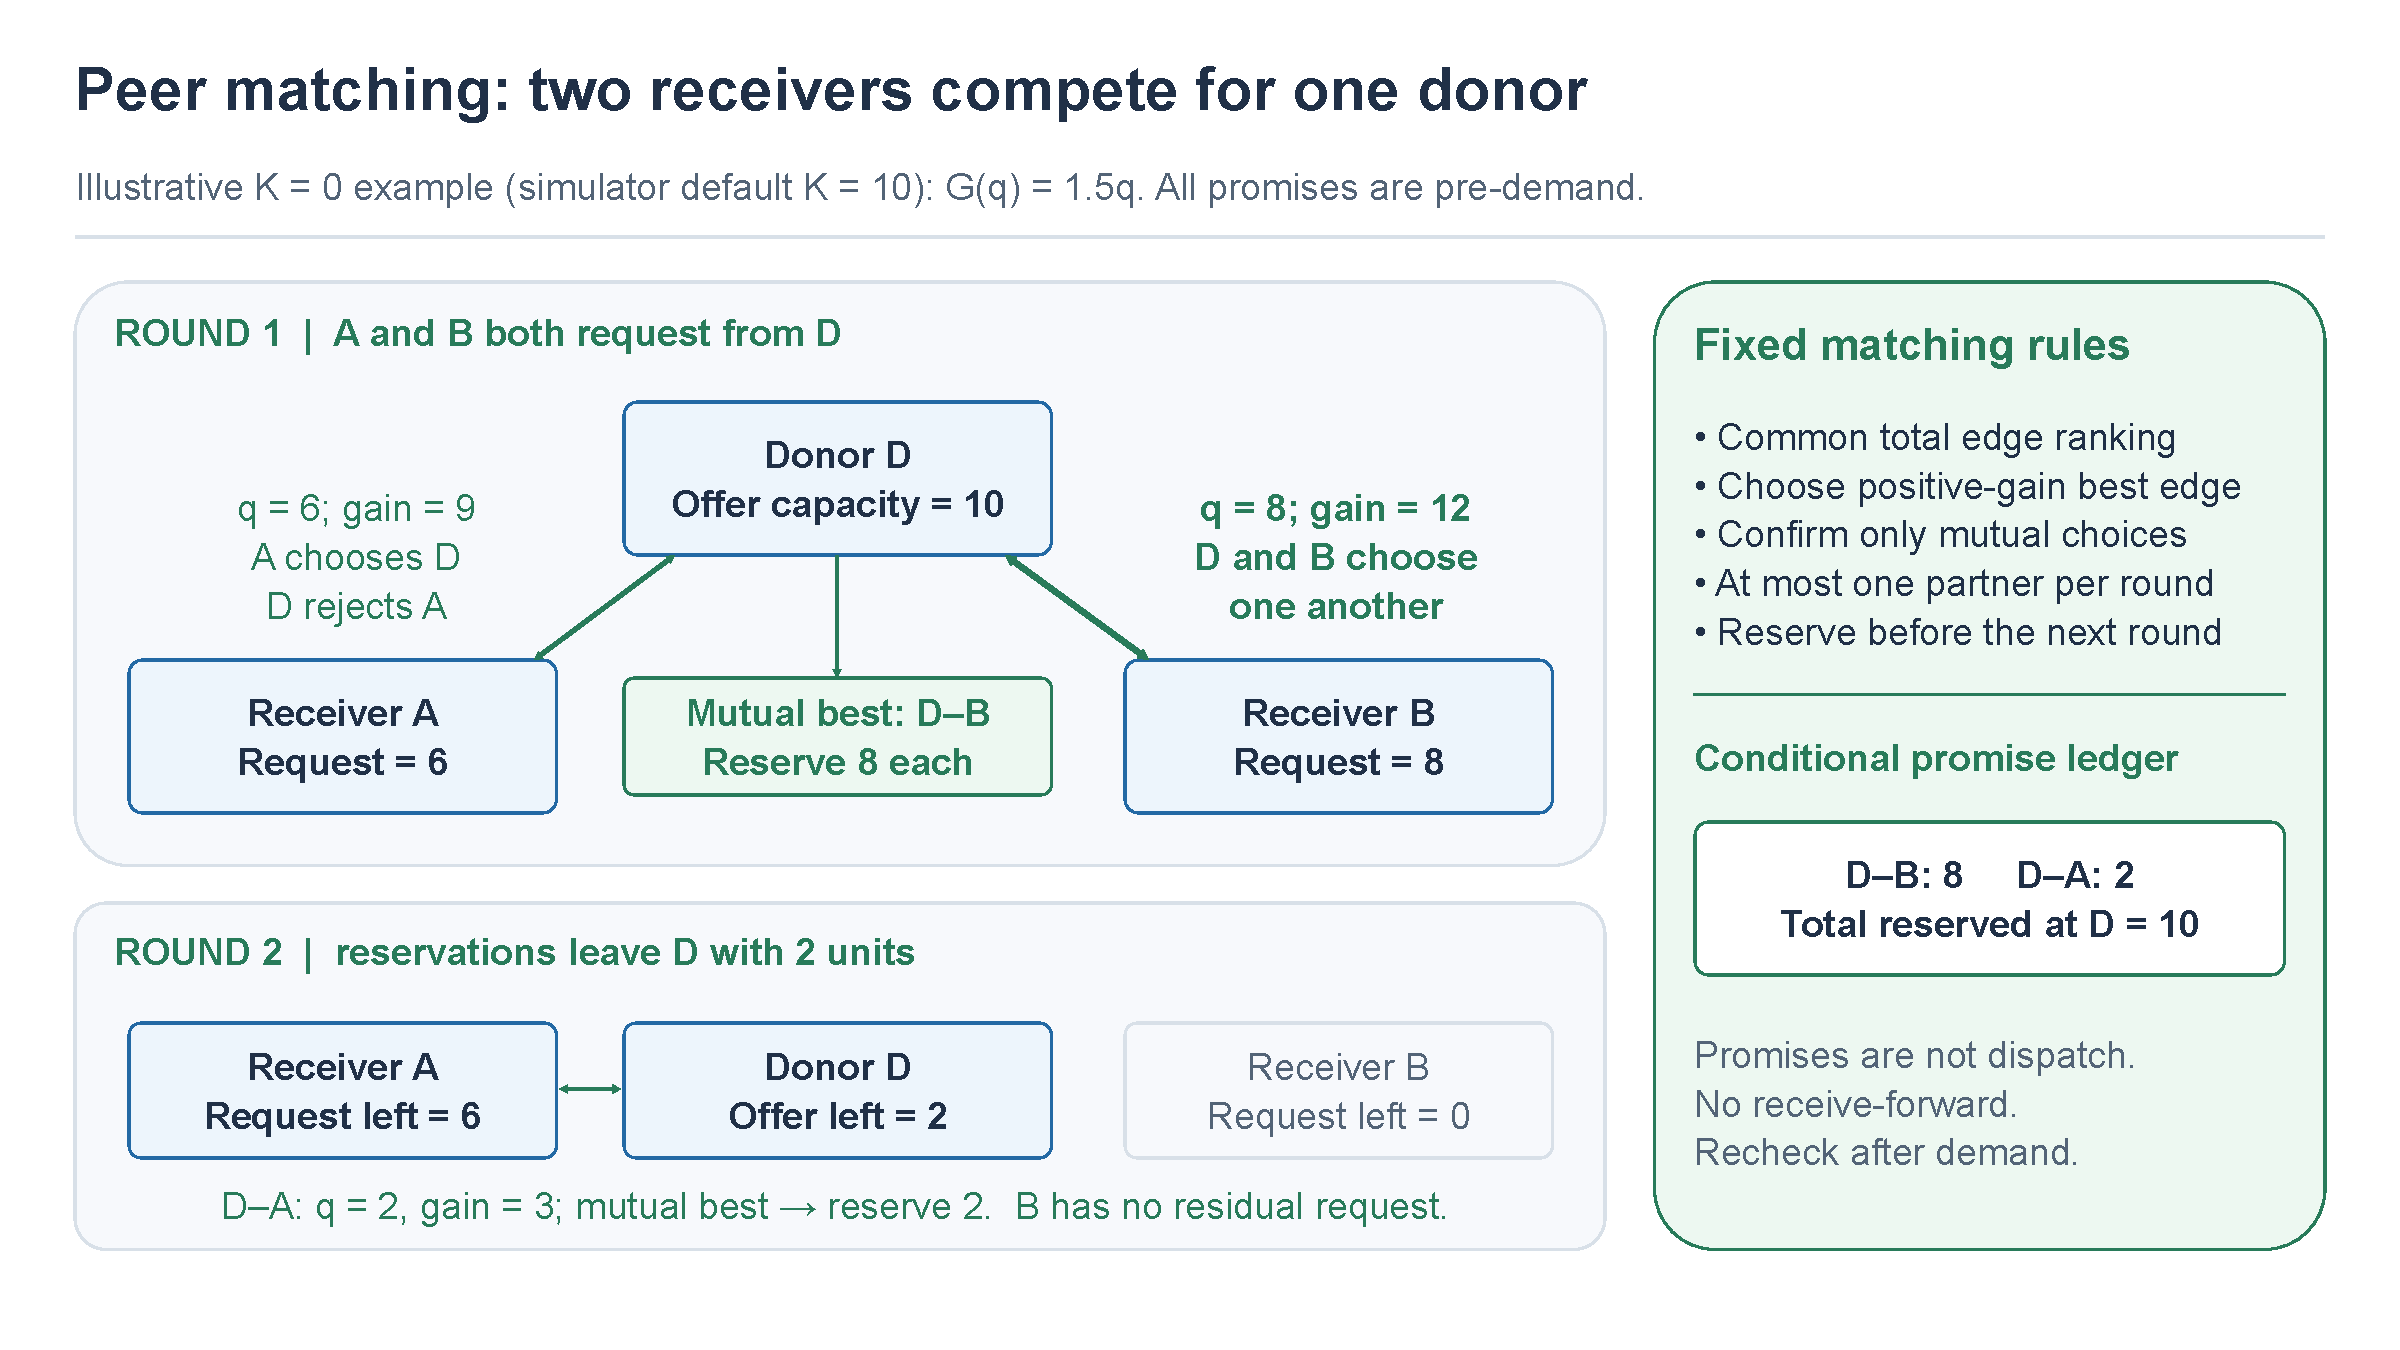
\includegraphics[width=0.96\textwidth]{figures/gp_agent_skills/negotiation.pdf}
    \caption{Peer negotiation with competing support requests. Local partner
    choices and reservations replace a central matching decision. Multiple
    rounds allow a donor to allocate residual supply.}
    \label{fig:negotiation}
\end{figure*}

Ledger invariants bound total planned outgoing supply and planned incoming
requests by each site's advertised remaining budgets. They prevent duplicate
commitments; they do not guarantee that post-demand inventory can fulfill
every promise. No global optimality or network-consensus convergence theorem
is asserted.

\subsection{Reservation Invariants and Local Authority}
Write $\mathcal C$ for confirmed commitments in the current period.
For a donor and receiver respectively, remaining budgets are
\begin{align}
 \bar s_i &= s_i-\sum_{(i,j,q)\in\mathcal C}q,\\
 \bar r_j &= r_j-\sum_{(i,j,q)\in\mathcal C}q.
\end{align}
A new confirmation uses
$0<q\leq\min(\bar s_i,\bar r_j)$ and updates both endpoints together.
Starting from empty ledgers, induction over confirmations gives
\begin{equation}
 \sum_{(i,j,q)\in\mathcal C}q\leq s_i,\qquad
 \sum_{(i,j,q)\in\mathcal C}q\leq r_j.
\end{equation}
The first inequality concerns each donor separately and the second each
receiver separately. They are promise-budget invariants, not assertions
about inventory after future demand.

Effective slack is updated consistently with commitments:
donating $q$ subtracts $q$ from the donor's negotiation slack, while receiving
$q$ adds it to the receiver's negotiation slack. An offer/request message
does not itself reserve stock. A partner preference does not itself confirm
a transfer. Only a mutually accepted confirmation changes the reservation
ledger; only physical dispatch changes actual transfer memory.
This lifecycle prevents an agent from treating an unaccepted proposal as
already received material.

\subsection{Conditional Dispatch and Execution Memory}
After current demand and due arrivals become available to the environment,
the fixed executor processes commitments by negotiation round, donor ID,
and receiver ID, using
(\ref{eq:execution}). Negotiation is not retrospectively rerun with realized
demand. For every commitment, it records planned and dispatched quantities,
full/partial/cancelled status, and the reason for any reduction.
Only dispatched quantities update the actual transfer history.
Costs are charged on actual dispatches; an approved but cancelled promise
does not incur a fictitious physical transfer cost.

\begin{figure*}[t]
    \centering
    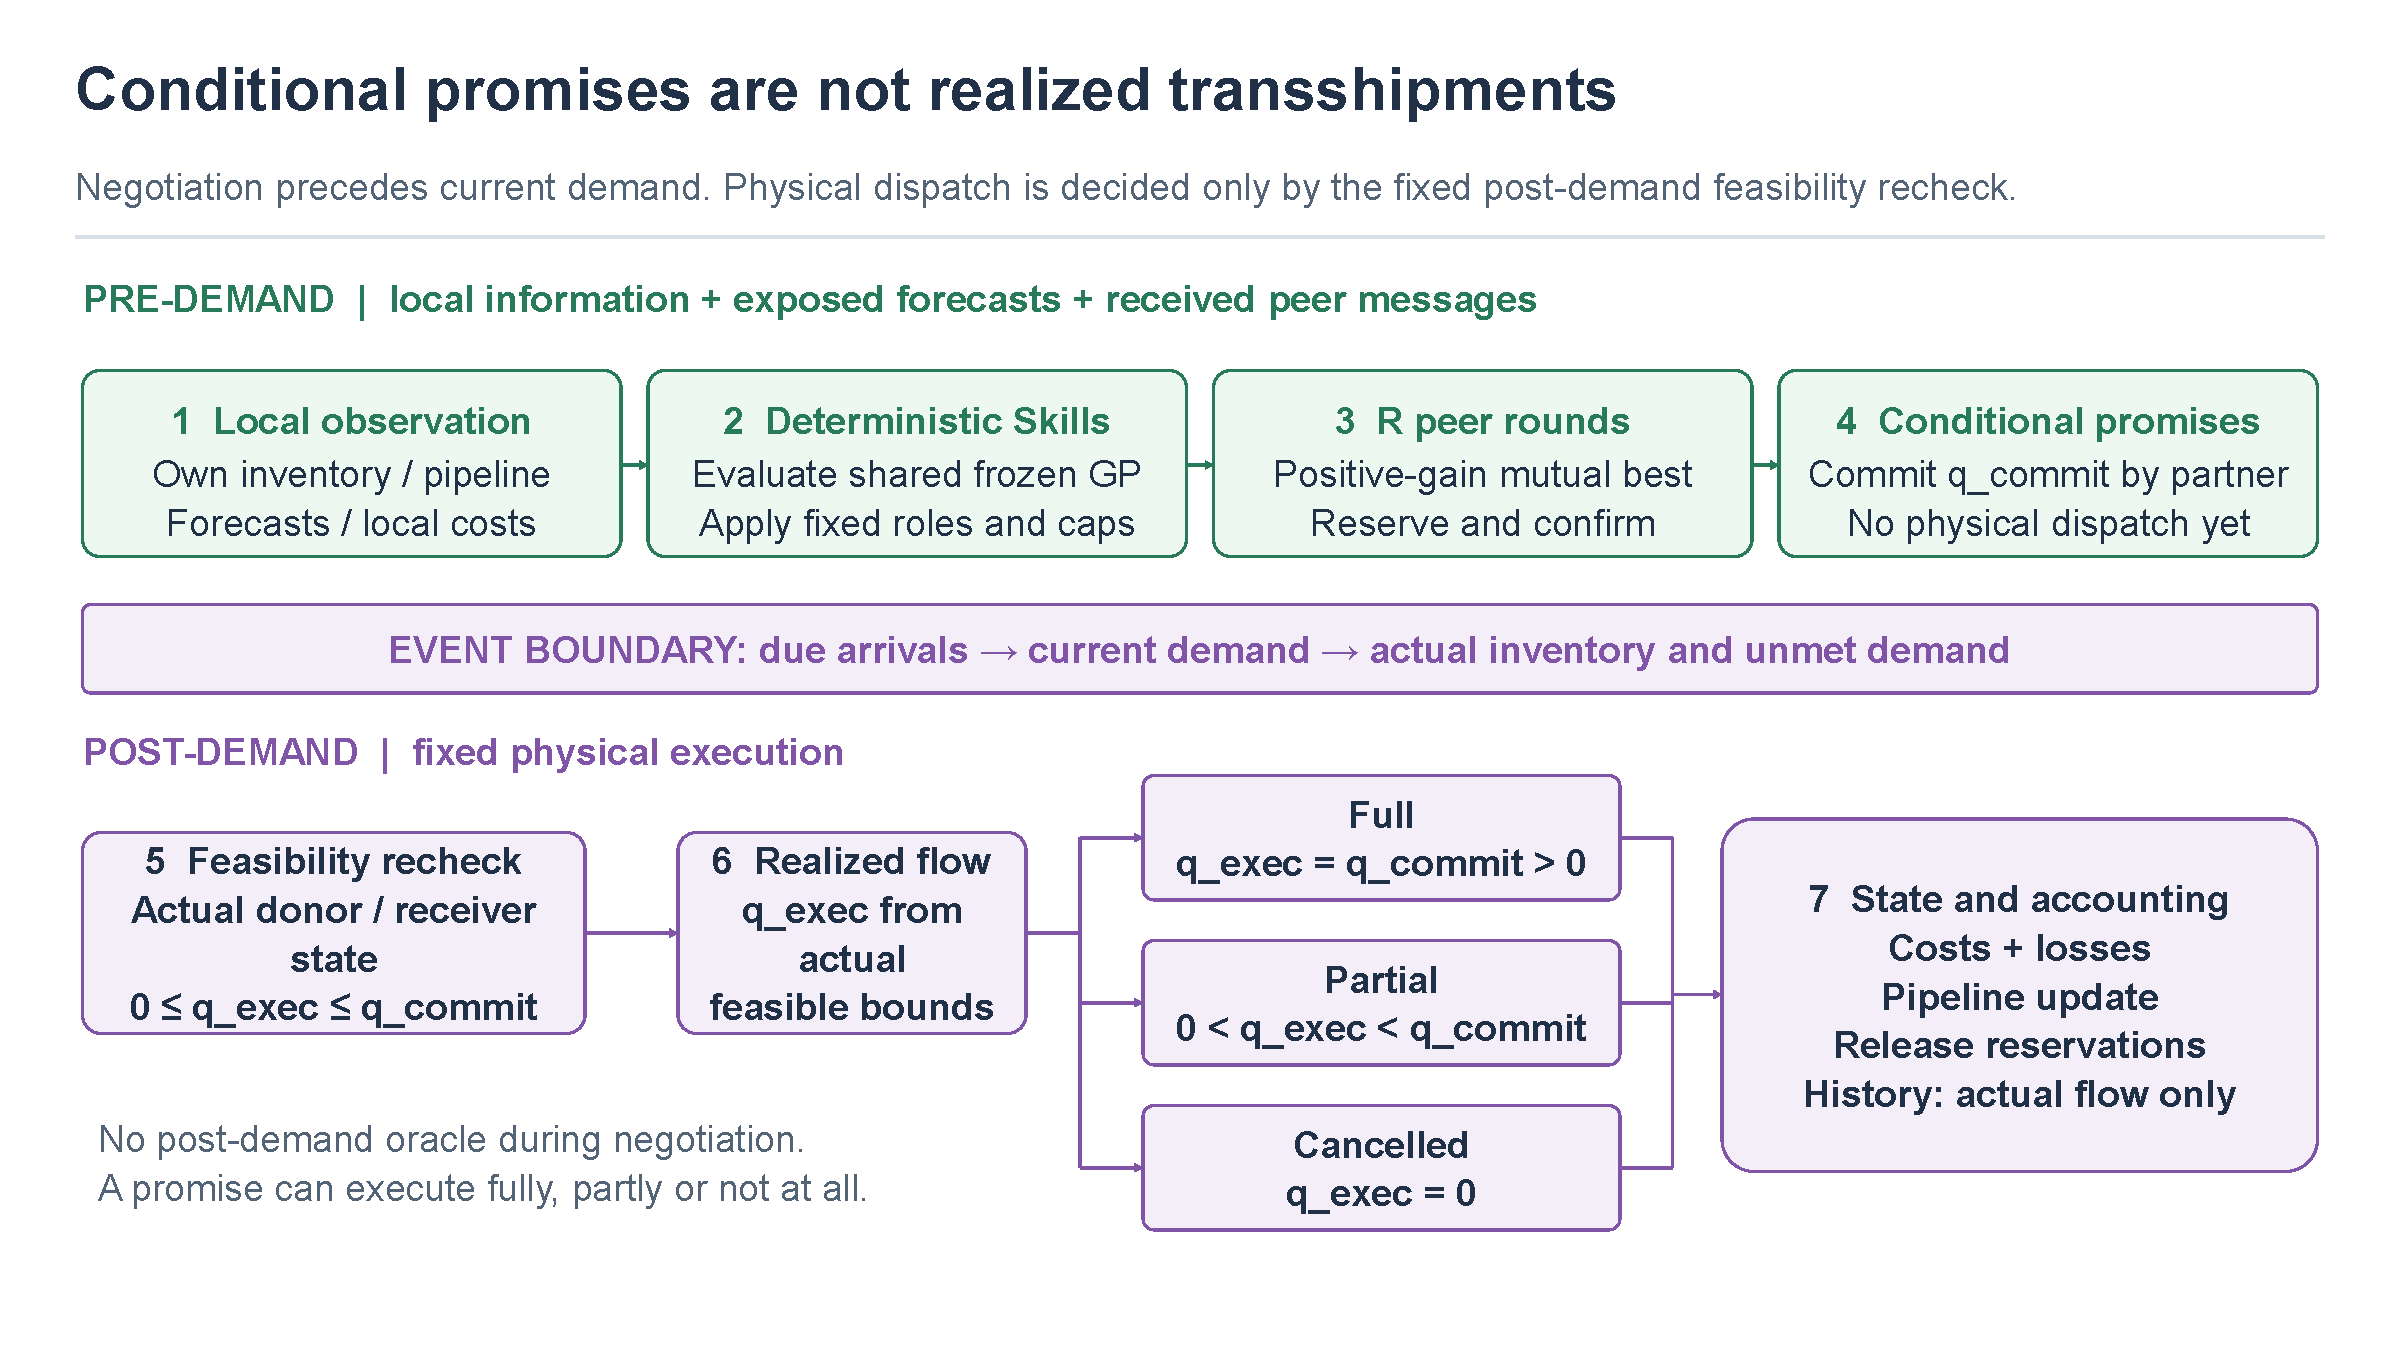
\includegraphics[width=0.96\textwidth]{figures/gp_agent_skills/timing.pdf}
    \caption{Pre-demand commitments and post-demand execution are separate
    events. Agents do not use future realized demand when negotiating.}
    \label{fig:timing}
\end{figure*}

\subsection{Offline GP Search and Fitness}
Initialization creates valid three-tree individuals, including interpretable
seed rules. The supplied seed consists of
\texttt{maximum(0.0, sub(F, add(I, PIPE)))},
\texttt{DEFICIT}, and \texttt{SURPLUS}, in order/request/offer order.
Tournament selection and elitism operate on
complete individuals. Crossover exchanges subtrees only between matching
roles; mutation changes one selected role's expression. Height/node limits
control bloat. The fixed negotiation and execution machinery is never
crossed over or mutated.

All competing candidates and retained elites use the same fixed training
scenario/seed batch across generations. This version does not rotate batches.
Unique generation champions form the candidates for selection on a disjoint
validation batch. The chosen policy is saved before held-out testing.
Let $D_{ei}$ and $L_{ei}$ be realized demand and final unmet demand for
site $i$ in episode $e$. Define
\begin{equation}
 \widehat{FR}_{ei}=
 \begin{cases}
  1-L_{ei}/D_{ei},&D_{ei}>0,\\
  1,&D_{ei}=0.
 \end{cases}
\end{equation}
With a common configured site service target $\tau$, exact batch fitness is
\begin{align}
  \mathcal F(\Theta)&=
  \left(V(\Theta),\overline J(\Theta),|\Theta|\right),\\
  V&=\max_e\sum_i\max(0,\tau-\widehat{FR}_{ei}),\\
  \overline J&=\frac{1}{M}\sum_{e=1}^{M}\frac{C_e}{T_e}.
\end{align}
There is no division of cost by site count. Smaller lexicographic values
are preferred; exact ties use canonical tree-string tuples. The service
constraint is site-wise, so a neglected site cannot be hidden by a high
network-aggregated fill rate. This remains empirical constraint handling,
not a statistical safety certificate.

\begin{table}[t]
\centering
\caption{Implemented search defaults}
\label{tab:search-defaults}
\footnotesize
\begin{tabular}{p{0.58\linewidth}p{0.32\linewidth}}
\toprule
Setting & Default \\
\midrule
Population / replacement generations & 20 / 5 \\
Tournament size / elites & 3 / 1 \\
Crossover / mutation / reproduction & 0.80 / 0.15 / 0.05 \\
Initial half-and-half depth & 0--2 \\
Mutation grow depth & 0--2 \\
Maximum height / nodes per tree & 5 / 63 \\
Negotiation rounds / site fill target & 3 / 0.95 \\
Training seeds & 11, 12 \\
Validation seeds & 1001, 1002 \\
Held-out seeds & 2001, 2002 \\
\bottomrule
\end{tabular}
\end{table}
Variation selects one homologous module. Structurally excessive children
revert to their corresponding parent. Search is serial; the smoke command
uses population six and one replacement generation without shortening the
default 64-period scenario. These are prototype defaults, not tuned
experimental budgets.

\begin{algorithm}[t]
\caption{Three-tree GP policy search}
\label{alg:gp}
\begin{algorithmic}[1]
\STATE Initialize population of $(T^{ord},T^{req},T^{off})$.
\STATE Evaluate the initial population on a common training batch.
\FOR{each generation}
    \STATE Rank the evaluated population by violation, cost, and size.
    \STATE Retain elites and select parents for offspring.
    \STATE Apply same-role crossover and module mutation.
    \STATE Enforce structural and numerical validity constraints.
    \STATE Evaluate offspring on the same current training batch.
    \STATE Form the next population from evaluated offspring and elites.
\ENDFOR
\STATE Select among unique generation champions on validation trajectories.
\STATE Freeze and serialize its three expressions and configuration.
\STATE Evaluate once on the held-out test protocol; deploy local skills.
\end{algorithmic}
\end{algorithm}

\begin{figure*}[t]
    \centering
    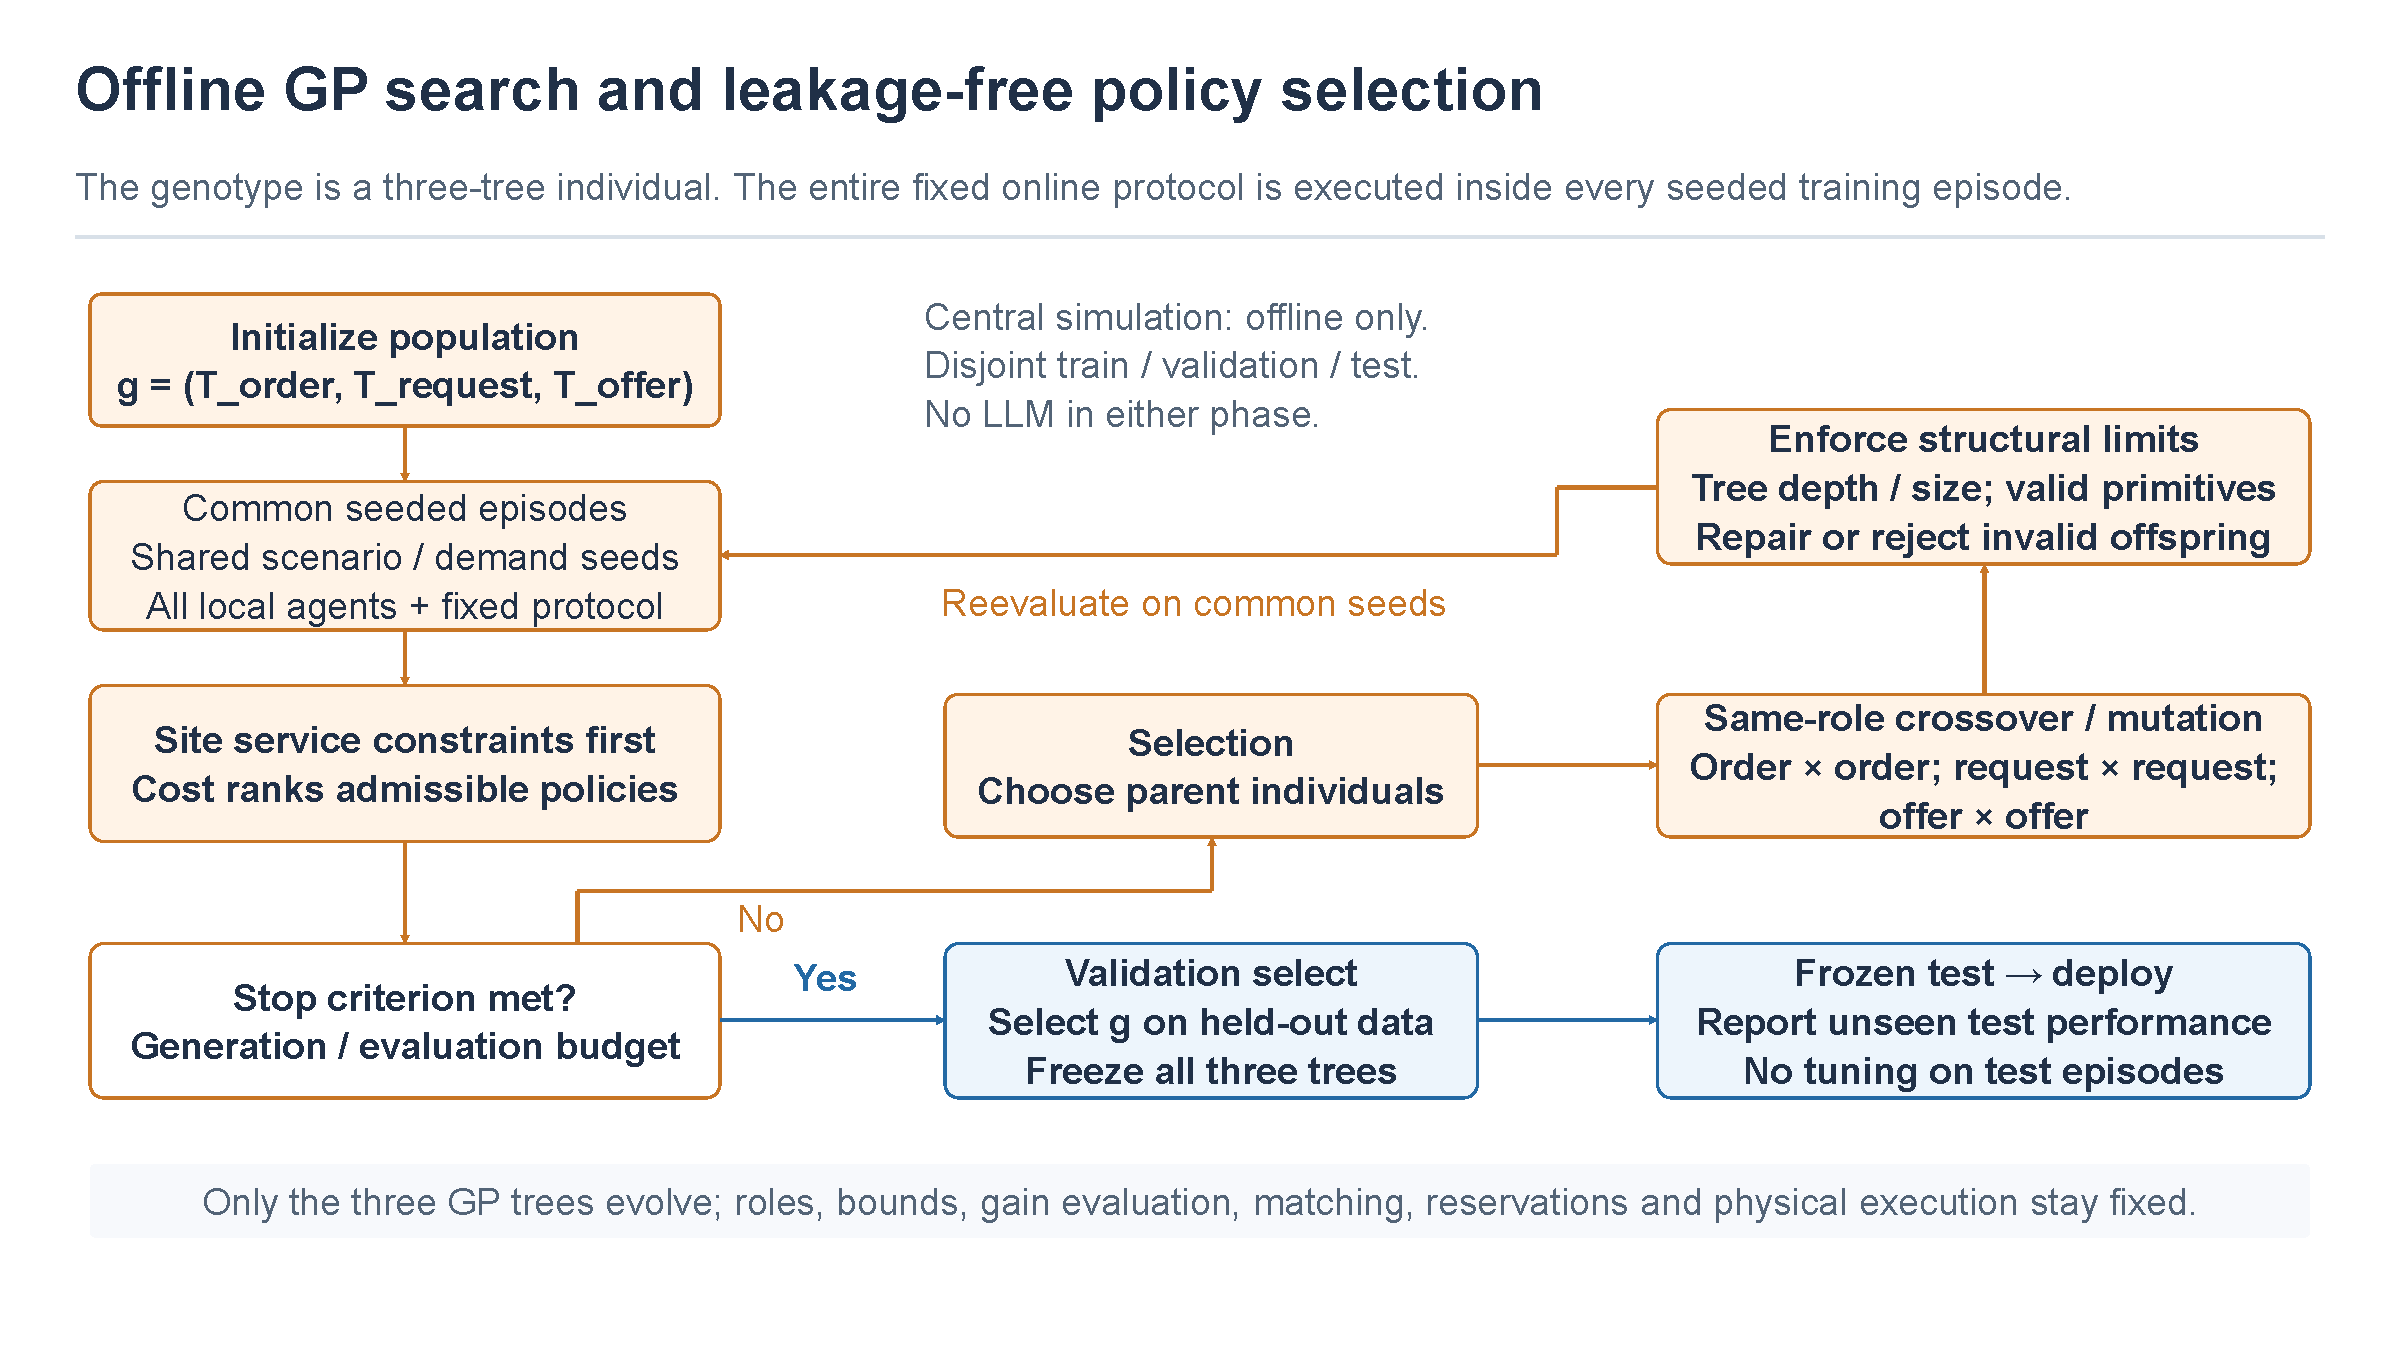
\includegraphics[width=0.96\textwidth]{figures/gp_agent_skills/gp_search.pdf}
    \caption{Offline GP search and separate validation/test evaluation.
    Deployment executes frozen expressions; it performs neither evolution nor
    LLM inference.}
    \label{fig:search}
\end{figure*}

\subsection{What Is Deliberately Not Learned}
This version does not evolve message syntax, communication topology,
quantity-grid definition, gain equations, matching protocol, or physical
constraints. It does not use five-tree value learning, partner-pool
coevolution, or counterfactual credit assignment. Those are separate
extensions requiring new ablations. Keeping these boundaries explicit makes
the first three-tree prototype reproducible and its empirical effects
attributable.

\subsection{Computational and Communication Structure}
Let $L$ be the total number of nodes in the three expressions and $K_q$ the
number of candidate quantities per edge. Local tree execution is linear in
the visited expression size. Across all sites and negotiation rounds, a
period requires on the order of
\begin{equation}
    O(NL+R|\mathcal E|K_q)
\end{equation}
arithmetic work, apart from state updates and physical execution.
Summary exchange, preferences, and confirmations require
$O(R|\mathcal E|)$ bounded-size messages in a synchronous implementation.
These are structural counts, not measured latency guarantees.
For a complete graph, $|\mathcal E|=N(N-1)/2$; parameter sharing alone
does not remove quadratic all-to-all communication. Sparse-topology and
round-budget experiments are therefore essential to any scalability claim.


\section{Evaluation Protocol}
\label{sec:evaluation}
This manuscript supplies an executable methods prototype, not a completed
comparative study. Training uses common scenario/seed batches across
competing individuals. Validation selects among candidate policies; final
test trajectories do not participate in selection. Demand repetitions
measure a frozen policy's variability and must not be counted as independent
GP search runs.

Required baselines include tuned local inventory rules, no lateral
transshipment, the copied two-tree replenish/transship GP, and the same
three-tree representation with independent pairwise acceptance instead of
mutual matching. A fixed hand-written request/offer policy isolates the
benefit of GP search from the benefit of the protocol. Information, timing,
action bounds/precision, scenario distribution, and simulation budgets must
be aligned. The new skill wrappers do not apply the legacy logistic action
map or its two-decimal rounding.

Ablations should vary negotiation rounds, graph connectivity, request/offer
evolution, and reservation handling. An unconstrained oracle-information
controller may be used as a reference, but is not automatically an optimal
bound. Stress tests should include multiple receivers competing for one
donor, asymmetric costs, demand shocks, and larger networks.

Report average cost and its components, per-site fill rate, unmet units,
planned and executed transfer quantities, full/partial/cancelled commitment
counts, and protocol communication. Report search wall time, episode
evaluations, tree sizes, independent search seeds, and paired test uncertainty.
Small smoke runs validate execution and reproducibility only; they cannot
establish an algorithmic advantage.

\section{Limitations and Conclusions}
Three-tree GP replaces a general code generator with a restricted symbolic
search space. The fixed protocol intentionally remains outside evolution,
which improves attribution but limits what coordination patterns can be
discovered. The gain proxy ignores much of the multi-period stochastic
problem; positive predicted gain is not a guarantee of positive realized
benefit. Shared rules do not establish performance with arbitrary
heterogeneous partners. Finite mutual matching need not solve the global
allocation problem, and conditional commitments can fail after demand.

The resulting research object is nevertheless precise: local inventory
agents use GP-parameterized skills to produce requests and offers; a fixed
peer protocol converts compatible choices into conditional commitments; a
separate executor enforces physical limits and records realized outcomes.
The next empirical task is to test whether this separation yields useful
cost--service tradeoffs under equal information and evaluation budgets.

\bibliographystyle{IEEEtran}
\bibliography{references}
\end{document}
